\subsection{Neural Networks}
Neural networks are built upon a simplified understanding of how the neurons in the brain function, wherein electrical impulses are passed in a chain reaction throughout the brain.
Feed-forward neural networks typically model this by passing an input through a composition of linear transformations and non-linear activation functions.
In a so-called \textit{feed-forward pass}, the input values $\boldsymbol{x} \in \mathbb{R}^{N_0}$ are sent to each neuron in the next layer, multiplied by a predetermined weight along the way with a value added called the bias $\boldsymbol{b} \in \mathbb{R}^{N_1}$.
We represent this through the function $\mathcal{A} : \mathbb{R}^{N_{i-1}} \to \mathbb{R}^{N_{i}}$ defined by
\begin{equation}
    \mathcal{A}_i(\boldsymbol{x}) = W_i \boldsymbol{x} + \boldsymbol{b}_i,
\end{equation}
where $W \in \mathbb{R}^{N_i \times N_{i-1}}$ is the weight matrix, where the $N_i$ is the number of neurons in layer $i$.
The resulting values are denoted $\boldsymbol{z}^i$.

The result of this is then passed through an activation function $\sigma_i : \mathbb{R} \to \mathbb{R}$, which we apply element-wise by $\boldsymbol{a}^i_j = \sigma_i (\boldsymbol{z}^i_j)$.
To simplify notation, we simply notate this as $\boldsymbol{a}^i = \sigma_i(\boldsymbol{z}^i)$.
This continues throughout each layer, culminating in the output layer, which in our case will simply have a the identity function as its activation function.
This process is illustrated in \autoref{fig:SimpleFFNN}.

\begin{figure}[h]
\centering
\def\layersep{2.5cm}
\def\nodeinlayersep{1.2cm}
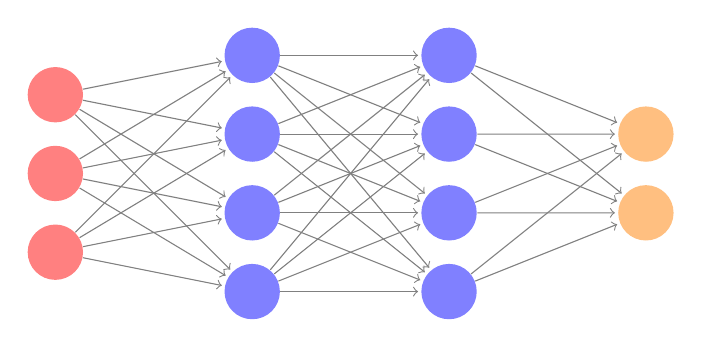
\begin{tikzpicture}[shorten >=1pt,->,draw=black!50, node distance=\layersep]
    \tikzstyle{every pin edge}=[<-,shorten <=1pt]
    \tikzstyle{neuron}=[circle, fill=black!25,minimum size=20pt,inner sep=0pt]
    \tikzstyle{input neuron}=[neuron, fill=red!50];
    \tikzstyle{output neuron}=[neuron, fill=orange!50];
    \tikzstyle{hidden neuron}=[neuron, fill=blue!50, minimum size=20pt];
    \tikzstyle{hidden neuron2}=[neuron, fill=blue!50, minimum size=20pt];

    \foreach \name / \y in {0,...,2}
        \node[input neuron] (I-\name) at (0,-\y) {};

    \foreach \name / \y in {0,...,3}
        \path[yshift=0.5cm]
            node[hidden neuron] (H1-\name) at (\layersep,-\y cm) {};

    \foreach \name / \y in {0,...,3}
        \path[yshift=0.5cm]
            node[hidden neuron2] (H2-\name) at (2*\layersep,-\y cm) {};    

    \foreach \name / \y in {0,...,1}
        % \node[output neuron,pin={[pun edge={->}]right:Output \#\y}, right of=H2-2] (O-\name) at (3*\layersep, -\y cm) {};
        \path[yshift=-0.5cm]
            node[output neuron] (O-\name) at (3*\layersep, -\y cm) {};


    \foreach \source in {0,...,2}
        \foreach \dest in {0,...,3}
            \path (I-\source) edge (H1-\dest);

    \foreach \source in {0,...,3}
        \foreach \dest in {0,...,3}
            \path (H1-\source) edge (H2-\dest);

    \foreach \source in {0,...,3}
        \foreach \dest in {0,...,1}
            \path (H2-\source) edge (O-\dest);
\end{tikzpicture}
\caption{Illustration of a fully connected feed-forward neural network with an input layer (red), two hidden layers (blue) and an output layer (orange).}
\label{fig:SimpleFFNN}
\end{figure}

Let $\boldsymbol{\theta} = \{ W_i, \boldsymbol{b}_i \}_{i = 1}^L$ represent the trainable parameters of the network in the parameter space $\mathcal{V}$, and $\mathcal{N}_{\boldsymbol{\theta}} : \mathbb{R}^{N_0} \to \mathbb{R}^{N_L}$ denote the realization of a neural network with $L$ layers, defined by
\begin{equation}
\begin{split}\label{eq:NNreal}
    \mathcal{N}_{\boldsymbol{\theta}} &= \sigma_L \circ \mathcal{A}_L \circ \sigma_{L-1} \circ \ldots \circ \sigma_{1} \circ \mathcal{A}_1 \\
    &= \bigcirc_{i = 1}^L \sigma_i \circ \mathcal{A}_i.
\end{split}
\end{equation}
We call the parameters trainable, as we typically initialize them to random values, \textit{training} them through optimization with the help of the backpropagation algorithm.
We do this by measuring how well our model is able to predict a set of values with a cost function $\mathcal{C}$, which often gives the problem the form of finding
\begin{equation}\label{eq:argmintheta}
    \hat{\boldsymbol{\theta}} = \argmin_{\boldsymbol{\theta} \in \mathcal{V}} \mathcal{C} \left( \mathcal{N}_{\boldsymbol{\theta}}, \boldsymbol{x}, \boldsymbol{\hat{y}} \right),
\end{equation}
where $\boldsymbol{\hat{y}} \in \mathbb{R}^{N_L}$ are a set of target values.

A typical choice of $\mathcal{C}$ in a regression problem is the Mean Squared Error (MSE), defined by
\begin{equation}
    \mathcal{C}(\mathcal{N}_\theta, \boldsymbol{x}, \boldsymbol{y}) = \frac{1}{n} \lVert \mathcal{N}_\theta(\boldsymbol{x}) - \boldsymbol{y} \rVert_2^2.
\end{equation}
One of the main benefits of this measure is its ease of differentiation, lightening the computational load of training the network.

Through the Universal Approximation theorem, first proven by \textcite{Cybenko1989ApproximationBS} and since extended, neural networks have a proven capacity to approximate any given function.
It does not state however how one is to find the architecture and parameters which solve a given problem.
The theorem does however guarantee the validity of at least attempting to utilize neural networks in a number of fields.

\subsection{Partial Differential Equations}
A Partial Differential Equation (PDE) is defined to be an equation containing a function with at least two different variables, as well as some degree of partial derivatives to these variables.
PDEs are ubiquitous in describing the properties, behavior, and evolution of physical systems.
A prime example is Poisson’s equation, which is of broad utility within theoretical physics. It is defined by
\begin{equation*}
    u_{xx} + u_{yy} = f \text{ on }\Omega,
\end{equation*}
where the residual $f$ is independent of $u$, and your domain $\Omega \in \mathbb R ^d$, where d is your number of dimensions, including a possible temporal dimension. 

An important concept when discussing PDEs is differential operators.
A differential operator is defined as a function of the differentiation operator.
It is indeed a function from a function space $\mathcal{F}_1$ to another function space $\mathcal{F}_2$.
In the case of a function of $n$ variables $u(x_1, x_2, \ldots , x_n)$ the usual differential operator is defined as 
\begin{equation*}
    D^\alpha u = \frac{\partial u^{|\alpha|}}{\partial x_1^{\alpha_1} \partial x_2^{\alpha_2} \cdots \partial x_n^{\alpha_n}},
\end{equation*}
where $|\alpha| = \alpha_1 + \alpha_2 + \ldots + \alpha_n$.
When considering a function $u(x,y)$, we will denote $\frac{\partial u}{\partial x}$ as $u_x$, $\frac{\partial^2 u}{\partial x^2}$ as $u_{xx}$, $\frac{\partial u}{\partial y}$ as $u_y$ and so on.
We will when discussing general PDEs denote the differential operator characterizing the PDE by $\mathcal{L}$.
For example, for the Poisson equation mentioned above, we have $\mathcal{L}u = u_{xx} + u_{yy}$, and denote the equation as $\mathcal{L}u=f$.
We will also come across the differential operator $\nabla$ (nabla).
For a problem in three physical dimensions, nabla is defined as $\nabla = \frac{\partial}{\partial x}\boldsymbol{x} + \frac{\partial}{\partial y}\boldsymbol{y} + \frac{\partial}{\partial z}\boldsymbol{z}$, where $\boldsymbol{x},\boldsymbol{y},\boldsymbol{z}$ are the three-dimensional Euclidean unit vectors.

When considering time-dependent PDEs for physical problems, we frequently require initial- and boundary conditions.
Initial conditions are conditions for values at $t=0$, and boundary conditions are value conditions at the physical boundary of the problem. Thus, both conditions are defined on the boundary $\partial\Omega$ of our spatial-temporal domain, and we treat them similarly.
In this paper we encounter Dirichlet-type boundary conditions (also referred to as first-type boundary conditions), that is when the value of the function on the boundary is given.
We return to the Poisson equation as an example;
we have for the function $u(x,y)$, $(x,y) \in [0,1]\times [0,1]$ the boundary conditions $u(0,y)=u(1,y)=u(x,0)=u(x,1) = 0$.
Another important is Neumann (or second-type) boundary conditions.
This is when the boundary conditions gives the value of the first order derivative of in the direction normal to the boundary. 

To capture these boundary conditions, we introduce a boundary value operator $\mathcal B$ such that we can write $\mathcal B u = g \text{ on }\partial \Omega$ for all our boundary conditions, for some function $g$ on the boundary $\partial\Omega$.

Given the PDE operator $\mathcal L$ and the boundary value operator $\mathcal B$, we present the general form of a PDE as:
\begin{equation}
\begin{cases}
    \mathcal{L}u &= f \textbf{ in }\Omega,\\
    \mathcal{B}u &= g \textbf{ in }\partial\Omega,    
\end{cases}
\label{eq:PDE}
\end{equation}

\subsection{Physics-Informed Neural Networks}
Physics-Informed Neural Networks (PINNs) incorporate the inherent physical constraints of a problem directly into the network.
One such way is to bake in the PDE conditions of a problem directly into the loss function of the network \cite{RAISSI2019686}
In doing so, we coerce the network into predicting results which adhere to the inherent physical laws.
In this way, we reduce the need for labeled data, and are able to be more confident in the predictions of our network.
Our neural network $\mathcal{N}_{\boldsymbol{\theta}}$ can then be regarded as an approximation of the hidden function $u$, notating it as $u^*$.

We then measure the loss through
\begin{equation}\label{eq:PINNMSE}
    \MSE = \MSE_d + \MSE_0 + \MSE_u + \MSE_f,
\end{equation}
where
\begin{equation*}
\begin{split}
    \underbrace{\MSE_d}_{\text{data}} &= \frac{1}{N_d} \sum_{i = 0}^{N_d} \left( u^*(x_d^i) - u_d^i \right)^2,  \\
    \underbrace{\MSE_0}_{\text{Initial}} &= \frac{1}{N_0} \sum_{i = 0}^{N_0} \left( u^*(x_0^i) - u_0^i \right)^2,  \\
    \underbrace{\MSE_u}_{\text{Boundary}} &= \frac{1}{N_u} \sum_{i = 0}^{N_u} \left( u^*(x_u^i) - g(x_u^i) \right)^2, \\
    \underbrace{\MSE_f}_{\text{Residual}} &= \frac{1}{N_f} \sum_{i = 0}^{N_f} \left( \mathcal{L}u^*(x_f^i) - f(x_f^i) \right)^2.
\end{split}
\end{equation*}
In this case, $(x_d^i,u_d^i)_{i=1}^{N_d}$ is a sample of data, $u_0^i$ is our initial condition, and $N_d,N_0,N_u,N_f$ is the number of data-, initial-, boundary-, and residual points on which the loss is calculated respectively. 
With this baseline, one can extend the loss function through appending more terms, if there are other conditions, such as periodicity, one would like to enforce.
Note that in $\MSE_f$, we are taking the derivative of the network itself with respect to its output.
This is done through the use of automatic differentiation, in much the same way the parameters are optimized.


The total process of applying machine learning techniques can then be quite beneficial, as the process of accruing data, whether that be with measurements, numerically or analytically, can be extremely costly.
In addition, with a framework already set up, the process of setting up a PINN is quite simple, in contrast to developing a numerical algorithm.

\subsection{Extended Physics-Informed Neural Networks}
Extended Physics-Informed Neural Networks (XPINNs), is a generalized space-time domain decomposition algorithm for PINNs initially proposed in \textcite{Jagtap2020ExtendedPN}.
The key idea is to decompose the domain $\Omega$ into several sub-domains $(\Omega_s)_s^N$ such that $\bigcup_{s=1}^{N_\mathrm{sd}}\Omega_s=\Omega$.
\textcolor{red}{NEED FIGURE}.
The domain interfaces are given by $\Omega_i\cap \Omega_j = \partial\Omega_{ij},\, i\neq j$.
Each sub-domain is then equipped with its own sub-PINN $u^*_s$, and the training and test points associated with its subdomain. 

Given such a domain decomposition, we now consider the following XPINN solution to our PDE problems:
\begin{equation}\label{eq:XPINN}
    u^* (x)=\sum_{s=1}^{N_\mathrm{sd}} u_{s}^*(x) \mathds{1}_{\Omega_s}(x),
\end{equation}
where $\mathds{1}_{\Omega_s}(x)$ is the indicator function given by:
\begin{equation}
    \mathds{1}_{\Omega_s}(x)=
    \begin{cases}
        0 &\text{If } x \notin \Omega_s \\
        1 &\text{If } x \in \Omega_s \backslash \text{common interface in } \Omega_s \\
        \frac{1}{S} &\text{If } x \in \text{common interface in } \Omega_s,
    \end{cases}
\end{equation}
where $S$ is the number of subdomains intersecting in the common interface.

A classical problem when applying domain decomposition is ensuring sufficient communication between the different subdomains such that their solutions reflect a global solution.
Ideally, the domain decomposition solution should be ``blind" to the decomposition.
For classical solvers, we frequently introduce \textit{ghost layers} to facilitate the communication between neighboring subdomains. 

However, as PINNs are mesh-independent we do not require ghost layers to communicate between PINNs.
XPINNs instead proposes to amend an additional \textit{interface loss} term $\MSE_I$ to the loss function \eqref{eq:PINNMSE} of each PINN to ensure that the PINNs agree on the subdomain interfaces.
For instance, we might wish to enforce continuity in our solution across an interface.
For a single PINN, we amend the loss function with
\begin{equation}\label{eq:MSE_I}
    \underbrace{\MSE_I}_{\text{Interface}} = \frac{1}{N_I} \sum_{i = 0}^{N_d} \left( u^*(x_I^i) - \{u_I^i\} \right)^2,  \\
\end{equation}
where $\{u_I^i\}$ is the average predicted value at the interface from each PINN, and $N_I$ is the number of points on the interface. 

\subsubsection{Use case of XPINNs}
Like traditional domain decomposition algorithms, XPINNs introduce an intuitive parallelization by separating the domain into several subdomains with their own respective neural network where the subdomain solutions can be computed on independent processors.
Thus, XPINNs might improve the computational efficiency through improved utilization of the processor architecture in a computer.

Moreover, \cite{Jagtap2020ExtendedPN} argue that XPINNs also introduce architectural flexibility into our problem.
For instance, we might employ a deep network in a subdomain with complex solution, whereas we can apply a shallow network for a subdomain with relatively simple and smooth solutions. 

However, the domain decomposition introduces a tradeoff for generalization.
On the one hand, we can leverage the architectural flexibility of XPINNs to decompose a complex PDE solution into several simple parts, decreasing the problem complexity and boosting generalization.
On the other hand, decomposing leads to each subdomain having access to less training data, which might cause overfitting and worse performance overall.
However, in an unsupervised setting, the computational load can be balanced through introducing more points in a previously lighter subdomain.
For a more rigorous analysis of when XPINNs improve generalization, we refer the reader to \cite{XPINN_generalize}.

Furthermore, the interface conditions also introduce complications to the loss function, changing the loss landscape.
Thus, it is easy to imagine instances where for instance the loss landscape of interface loss and boundary loss are different, resulting in an optimization dilemma of which condition to prioritize.
Moreover, changing the loss function through interface conditions might also correspond to altering the PDE problem equation.
To the extent of the authors' knowledge, there is not a clear theoretical understanding of how the interface conditions alter the solution to our PDE problem. 


